\documentclass[6pt]{../../shared/AiTex}
\usepackage{csvsimple}

\title{Memoria entrega 4}
\author{A.L.K.}
\date{Febrero 2024}

\begin{document}
%\datos{facultad}{universidad}{grado}{asignatura}{subtitulo}{autor}{curso}
\datos{Informática}{Universidad Complutense de Madrid}{Ingeniería informática}{Aprendizaje Automatico y Big Data}{Entrega 5: entrenamiento de redes neuronales}{Alejandro Barrachina Argudo}{2023-2024}
% \portadaApuntes
% \pagestyle{empty}
% \tableofcontents
% \pagestyle{empty}
\justify

\begin{center}

    {\huge \textbf{\underline{\subtitulo}}} \\
    { \lesson - \autor}

\end{center}


\section*{Introducción}

En este documento se explicará el código del entregable 5 y el proceso de entrenamiento de redes neuronales.

Para esta práctica se usarán los siguientes \textit{imports} vistos en la figura \ref{fig:imports}. Parte del código se reutiliza de la práctica anterior.
\begin{figure}[H]
    \centering
    \lstinputlisting[firstline=1,lastline=7, style=custompython]{../nn.py}
    \caption{Código de las bibliotecas usadas}
    \label{fig:imports}
\end{figure}

\begin{figure}[H]
    \centering
    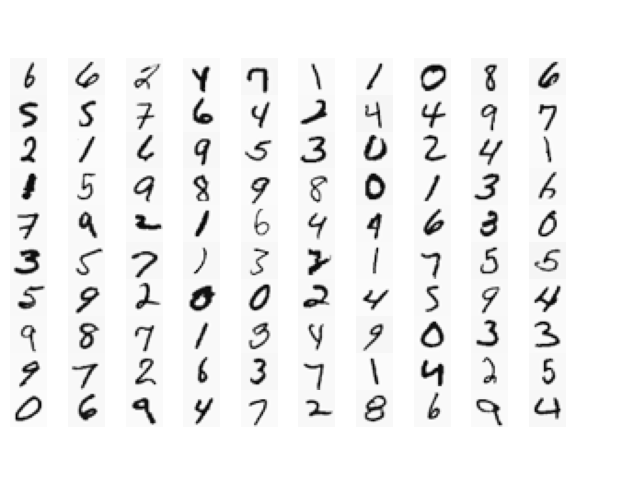
\includegraphics[width=0.5\textwidth]{./imagenes/dataset.png}
    \caption{Ejemplo de los dígitos del \textit{dataset}}
    \label{fig:digitos}
\end{figure}

\section{Entrenamiento de redes neuronales}

Para comprobar la red neuronal utilizaremos la función \textit{neural\_network} implementada en la figura \ref{fig:neural_network}. Esta función se implementa para un número indeterminado de capas.

Reimplementamos la función de coste (figura \ref{cost}) para que se adapte a las dos capas del ejercicio, esta función incluye también la regularización. La función de coste puede dar error para los números 0 y 1 por el uso del logaritmo, usamos la función \textit{fix\_data} (figura \ref{fig:fix_data}) para añadirle un infinitesimal valor para que no sea exactamente 0 o 1. Para la propagación primero haremos uso de la función de red neuronal para hacer la propagación hacia adelante y luego la propagación hacia atrás. Todo esto ocurre en la función \textit{backprop} que se muestra en la figura \ref{fig:backprop}.

Hacemos el descenso de gradiente en la función \textit{gradient\_descent} implementada en la figura \ref{fig:gradient_descent}. En esta función se hace uso de la función \textit{backprop} para calcular los gradientes y actualizar los pesos.

Para terminar usamos \textit{prediction}, \textit{predict\_percentage} y \textit{random\_init} como utilidades para el proceso de entrenamiento (figuras \ref{fig:prediction}, \ref{fig:predict_percentage} y \ref{fig:random_init}).

\begin{figure}[H]
    \centering
    \lstinputlisting[firstline=22,lastline=39, style=custompython]{../nn.py}
    \caption{Función \textit{neural\_network}}
    \label{fig:neural_network}
\end{figure}

\begin{figure}[H]
    \centering
    \lstinputlisting[firstline=42,lastline=91, style=custompython]{../nn.py}
    \caption{Función de coste}
    \label{cost}
\end{figure}

\begin{figure}[H]
    \centering
    \lstinputlisting[firstline=10,lastline=19, style=custompython]{../nn.py}
    \caption{Función \textit{fix\_data}}
    \label{fig:fix_data}
\end{figure}

\begin{figure}[H]
    \centering
    \lstinputlisting[firstline=94,lastline=165, style=custompython]{../nn.py}
    \caption{Función \textit{backprop}}
    \label{fig:backprop}
\end{figure}

\begin{figure}[H]
    \centering
    \lstinputlisting[firstline=168,lastline=192, style=custompython]{../nn.py}
    \caption{Función \textit{gradient\_descent}}
    \label{fig:gradient_descent}
\end{figure}

\begin{figure}[H]
    \centering
    \lstinputlisting[firstline=207,lastline=223, style=custompython]{../nn.py}
    \caption{Función \textit{prediction}}
    \label{fig:prediction}
\end{figure}

\begin{figure}[H]
    \centering
    \lstinputlisting[firstline=226,lastline=241, style=custompython]{../nn.py}
    \caption{Función \textit{predict\_percentage}}
    \label{fig:predict_percentage}
\end{figure}

\begin{figure}[H]
    \centering
    \lstinputlisting[firstline=195,lastline=204, style=custompython]{../nn.py}
    \caption{Función \textit{random\_init}}
    \label{fig:random_init}
\end{figure}

\section{Flujo de entrenamiento}

El programa llama a la función \textit{test\_learning} (figura \ref{fig:train_test}) que se encarga de entrenar la red neuronal. Primero codificamos y a la codificación \textit{one hot} mediante el uso de las funciones \textit{oneHotEncoding} y \textit{encoder} (figuras \ref{fig:oneHotEncoding}). Tras esto iniciamos los valores de iteración, número de capas, $\lambda$ y $\alpha$ e iniciamos aleatoriamente $\theta 1$ y $\theta 2$. Tras esto ejecutamos el descenso de gradiente, guardamos la matriz de confusión (usando la función de la práctica anterior) y guardamos los valores de la red neuronal usando la función \textit{save\_nn} (figura \ref{fig:save_nn}).

\begin{figure}[H]
    \centering
    \lstinputlisting[firstline=244,lastline=274, style=custompython]{../nn.py}
    \caption{Función \textit{test\_learning}}
    \label{fig:train_test}
\end{figure}

\begin{figure}[H]
    \centering
    \lstinputlisting[firstline=327,lastline=341, style=custompython]{../nn.py}
    \caption{Función \textit{oneHotEncoding}}
    \label{fig:oneHotEncoding}
\end{figure}
\begin{figure}[H]
    \centering
    \lstinputlisting[firstline=289,lastline=297, style=custompython]{../nn.py}
    \caption{Función \textit{save\_nn}}
    \label{fig:save_nn}
\end{figure}

\section{Funciones auxiliares y resultados}

Algunas funciones auxiliares del programa son las siguientes:
\begin{itemize}
    \item \textit{load\_nn} (figura \ref{fig:load_nn}): Carga los valores de la red neuronal.
    \item \textit{loadData} (figura \ref{fig:load_data}): Carga los datos del \textit{dataset}.
    \item \textit{loadWeights} (figura \ref{fig:load_weights}): Carga los pesos de la red neuronal de ejemplo.
    \item \textit{displayData} (figura \ref{fig:display_data}): Muestra los dígitos del \textit{dataset}.
    \item \textit{main} (figura \ref{fig:main}): Función principal del programa.
\end{itemize}

Podemos ver que la red neuronal consigue un 95\% de acierto, representado en la figura \ref{fig:resultado}.

\begin{figure}[H]
    \centering
    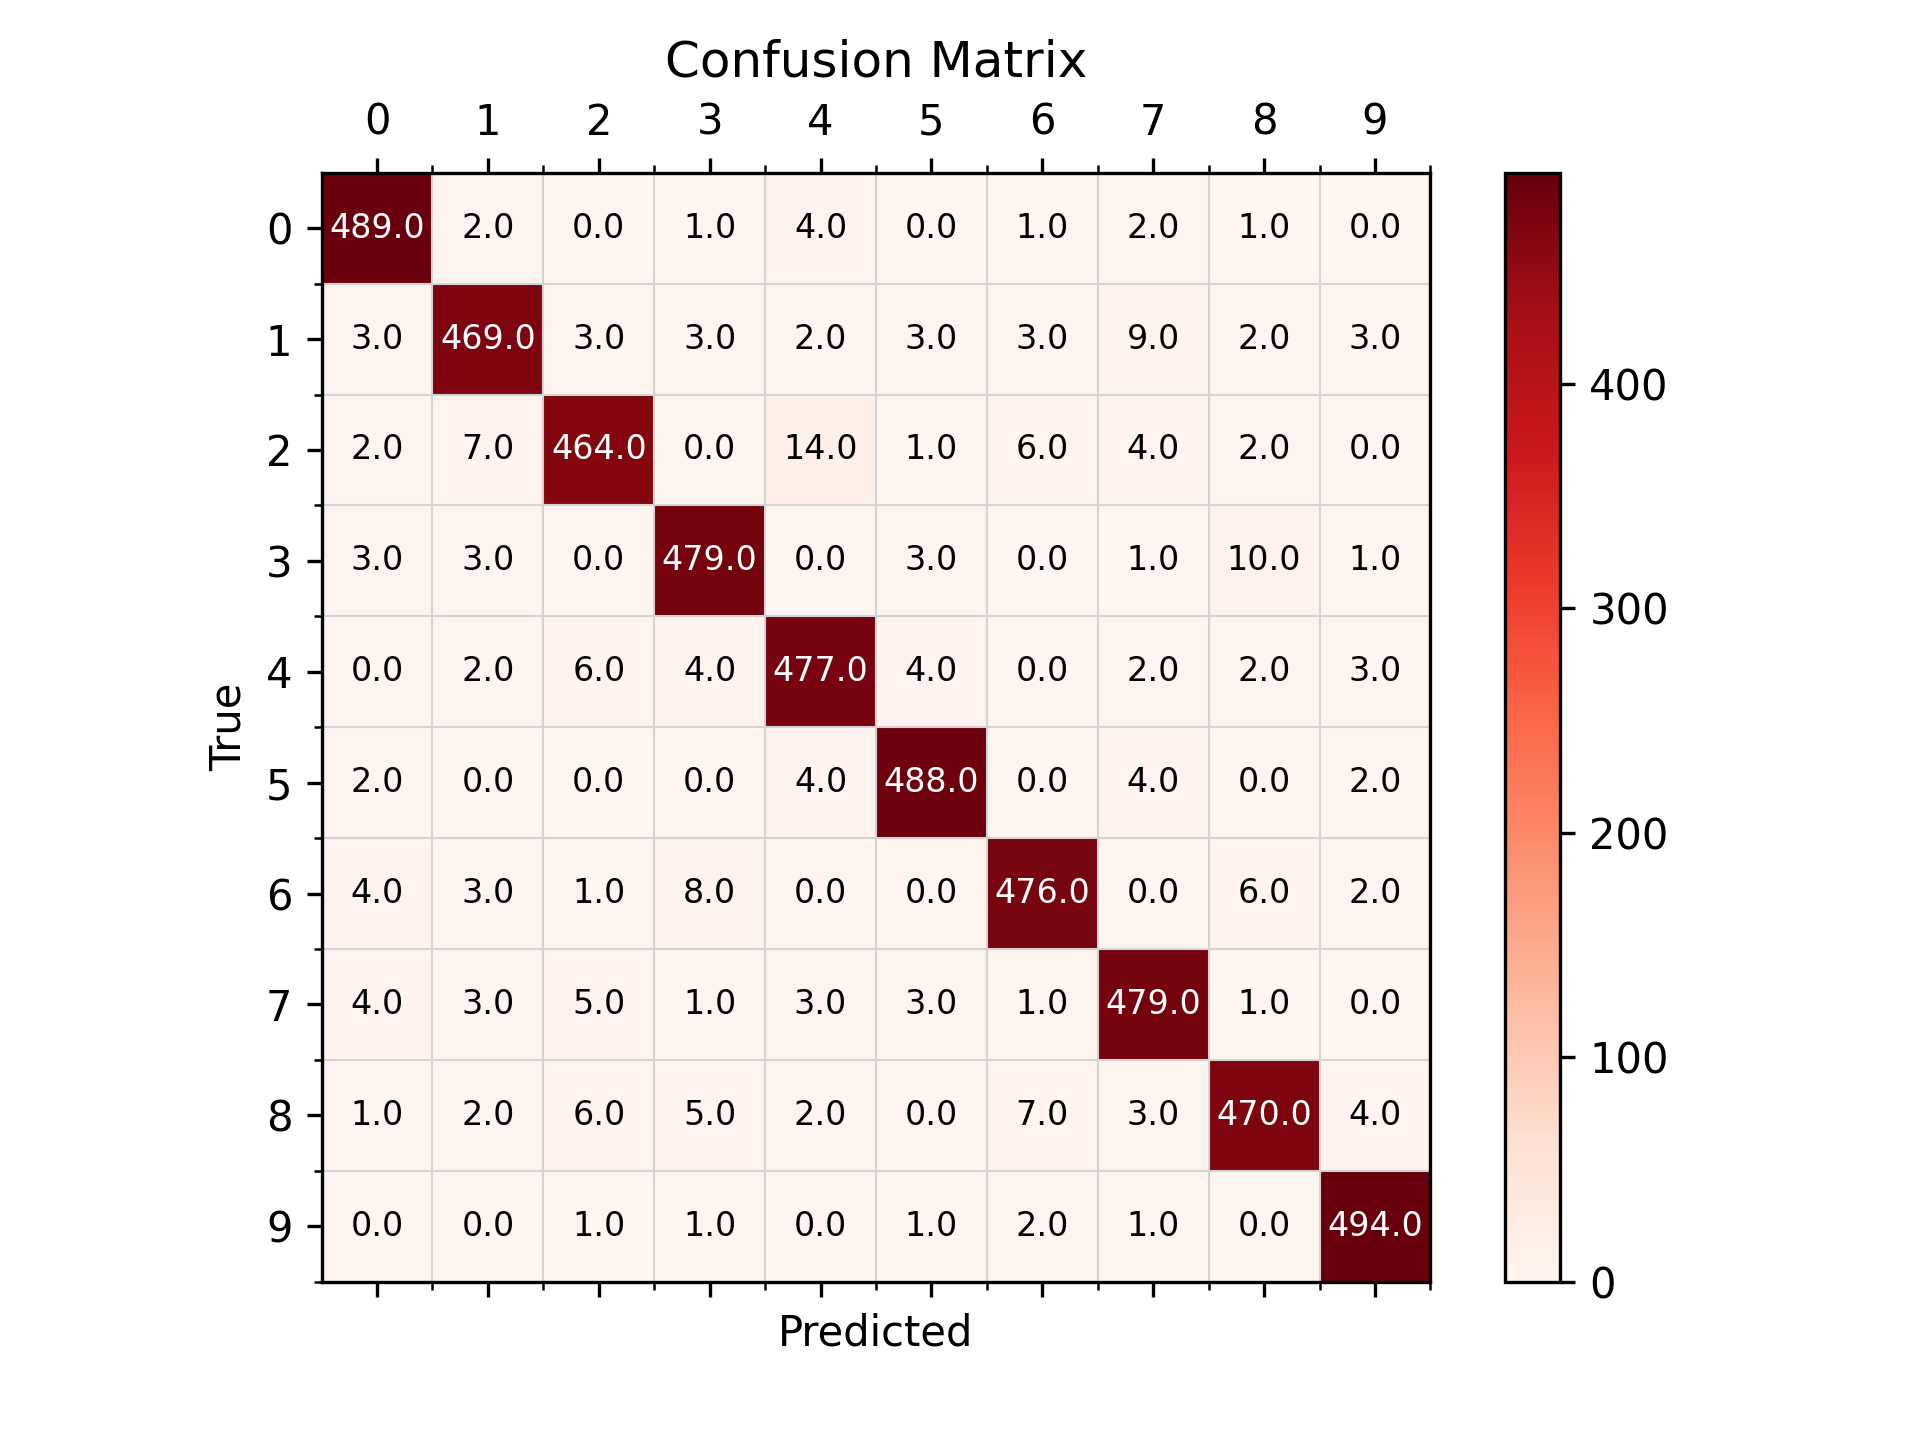
\includegraphics[width=0.5\textwidth]{./imagenes/confusion_matrix.png}
    \caption{Resultado de la red neuronal}
    \label{fig:resultado}
\end{figure}

\begin{figure}[H]
    \centering
    \lstinputlisting[firstline=300,lastline=312, style=custompython]{../nn.py}
    \caption{Función \textit{load\_nn}}
    \label{fig:load_nn}
\end{figure}

\begin{figure}[H]
    \centering
    \lstinputlisting[firstline=277,lastline=286, style=custompython]{../nn.py}
    \caption{Función \textit{loadData}}
    \label{fig:load_data}
\end{figure}

\begin{figure}[H]
    \centering
    \lstinputlisting[firstline=315,lastline=324, style=custompython]{../nn.py}
    \caption{Función \textit{loadWeights}}
    \label{fig:load_weights}
\end{figure}

\begin{figure}[H]
    \centering
    \lstinputlisting[firstline=344,lastline=354, style=custompython]{../nn.py}
    \caption{Función \textit{displayData}}
    \label{fig:display_data}
\end{figure}

\begin{figure}[H]
    \centering
    \lstinputlisting[firstline=357,lastline=382, style=custompython]{../nn.py}
    \caption{Función \textit{main}}
    \label{fig:main}
\end{figure}

\end{document}
